\section{Verstärkendes Lernen}
Verstärkendes Lernen oder als RL in der Fachsprache bezeichnet, definiert einen konzeptionellen Ansatz zielorientiertes Lernen von Entscheidungen zu verstehen und zu automatisieren. \footcite[Vgl.][S. 13]{Sutton.2018}
Dabei besteht der Fokus darauf das ein Agent aus der direkten Interaktion mit seiner Umgebung lernt, ohne das explizite Überwachung notwendig ist. \footcite[Vgl.][S. 13]{Sutton.2018}
Der Agent lernt über die Zeit eine optimale Strategie zur Lösung des Entscheidungsproblems aus dem Ausprobieren und Scheitern mittels verschiedener Aktionen die gewünschte Veränderung in seiner Umwelt herzustellen. \footcite[Vgl.][S. 4]{Li.2019}
Notwendig dabei ist es, das der Agent den Zustand seiner Umgebung wahrnehmen, und auch durch entsprechende Aktionen beeinflussen kann, sodass die Erreichung des Zielzustandes möglich ist. \footcite[Vgl.][S. 2]{Sutton.2018}
Zur Erreichung dieses Zielzustandes muss der Agent alle Aktionen entdecken, welche ihm die größtmögliche kumulierte Belohnung liefern, wobei Aktionen nicht nur die unmittelbare sondern auch zukünftige Belohnungen beeinflussen. \footcite[Vgl.][S. 1]{Sutton.2018}
%Damit grenzt RL sich vom überwachten Lernen in der Art und Weise ab, dass dem Agenten zwar evaluiertes Feedback zur Verfügung steht, jedoch keine direkte Kennzeichnung ob seine Aktion korrekt oder falsch war.\footcite[Vgl.][S. 4]{Li.2019} 
Zusammengefasst lässt sich die beschriebene Interaktion des Agenten mit seiner Umgebung wie folgt in Abbildung 1 darstellen.
\begin{figure}[htb]
    \centering
    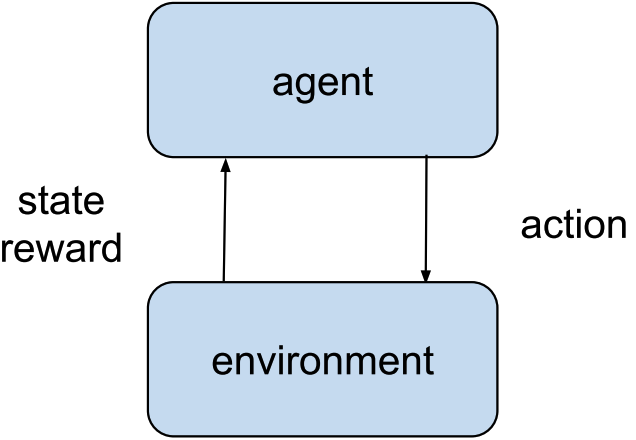
\includegraphics[height=4cm]{lib/graphics/Agent-Environment interaction.png}
    \caption[vereinfachte Darstellung der Interaktion zwischen dem Agenten und seiner Umgebung]{vereinfachte Darstellung der Interaktion zwischen dem Agenten und seiner Umgebung\footnotemark}
    \label{abb:Agent-Environment interaction}
\end{figure}
\footnotetext{Enthalten in: \cite[][S. 5]{Li.2019}}

Ein Standardaufbau einer Aufgabe für verstärkendes Lernen kann demnach verstanden werden, als sequentielles Entscheidungsproblem zu dessen Lösung ein Agent zu jedem diskreten Zeitschritt eine Aktion ausführt welche den Zustand der Umgebung verändert. \footcite[Vgl.][S. 2]{Zhao.2020}
Betrachtet man die technische Umsetzung einer solchen Interaktion zwischen dem Agenten und dessen Umgebung, wird häufig zur Modellierung ein Markov Entscheidungsprozess verwendet.
Im Kontext von RL ist der Entscheidungsprozess definiert nach einem Tupel aus folgenden sechs Elementen:\footcite[Vgl.][S. 2]{Zhang.2018}
\begin{itemize}
    \item Alle Zustände $S$
    \item Alle Aktionen $A$
    \item initiale Zustandsverteilung $p0(S)$
    \item Übergangswahrscheinlichkeit $T(S_{t+1}|S_{t},A_{t})$
    \item Belohnungswahrscheinlichkeit $R(r_{t+1}|S_{t},A_{t})$
    \item Abzinsungsfaktor $\gamma \in \left[0,1\right)$
\end{itemize}
Der Agent sucht in diesem Kontext die optimale Strategie $\pi_{\phi}$, welche allen Zuständen $S$ die jeweilige Aktion $A(S)$ zuordnet, sodass die kummulierte Belohnungswahrscheinlichkeit $R(r_{t+1}|S_{t},A_{t})$ über alle Zeitschritte $t$ maximal ist. \footcite[Vgl.][S. 2]{Reda.2020}

Neben dieser kurzfristigen direkten Belohnung müssen auch die langfristigen zukünftigen Belohnungen aus den neuen Zuständen betrachtet werden, wofür das Konzept der Wertigkeit eingeführt wird. \footcite[Vgl.][S. 3]{Wang.2020}
Über eine Zustands- oder Aktionswertigkeitsfunktion, oftmals als Q-Funktion referenziert, wird eine Vorhersage über die zu erwartende kumulierte abgezinste zukünftige Belohnung berechnet.\footcite[Vgl.][S. 5]{Li.2019}
Durch den Abzinsungsfaktor $\gamma$ wird der Einfluss zukünftiger Belohnungen nach ihrer zeitlichen Reihenfolge priorisiert.\footcite[Vgl][S. 5]{Li.2019}
Mit der Wertigkeitsfunktion kann evaluiert werden, welche Strategie langfristig am erfolgreichsten ist, da bspw. manche Aktionen trotz geringer sofortiger Belohnung einen hohen Wert aufweisen können, wenn aus dem zukünftigen Zustand eine hohe Belohnung zu erwarten ist.\footcite[Vgl.][S. 6]{Sutton.2018}
Die Wertigkeitsfunktion und die daraus berechneten Wertigkeiten von Aktionen oder Zuständen werden über alle Zeitschritte neu geschätzt und stellen mit die wichtigste Komponenten in Algorithmen des verstärkenden Lernens dar. \footcite[Vgl.][S. 6f.]{Sutton.2018}
Methoden basierend auf diesem Wertigkeitswert lernen eine Schätzfunktion der Wertigkeit für alle Zustände ($V_{\pi}(s) \forall S$) und alle Zustandsaktions-Paare ($Q_{\pi}(s_{t},a_{t}) \forall s,a \in (S,A)$) der optimalen Strategie $\pi$ durch aktualisieren der folgenden Funktionen: \footcite[Vgl.][S. 2]{Zhang.2018}
\begin{itemize}
    %\item 1: $Q(s_{t}, a_{t}| \omega_{t+1}) \leftarrow Q(s_{t}, a_{t}|\omega_{t}) + \alpha\left[r_{t+1} + \gamma\max\limits_{a}Q(s_{t+1},a|\omega)-Q(s_{t},a_{t}|\omega)\right]*\nabla_{\omega}Q(s_{t},a_{t}|\omega)$
    \item 1: $Q(s_{t}, a_{t}) \leftarrow Q(s_{t}, a_{t}) + \alpha\left[r_{t+1} + \gamma\max\limits_{a}Q(s_{t+1},a)-Q(s_{t},a_{t})\right]$
    \item 2: $V(s_{t}) = \max\limits_{a}Q(s_{t},a|\omega)$
\end{itemize}
Aus den geschätzten Wertigkeit jedes Zustandsaktions Paares kann die optimale Strategie $\pi^{*}(s)$ durch $\underset{a}{\arg\max}$ $Q(s,a)$ bestimmt werden. \footcite[Vgl.][S. 2]{Zhang.2018}

Neben den Methoden welche auf dem Konzept der Wertigkeit basieren können Strategie basierende Methoden die Strategie direkt durch bspw. ihren Gradienten optimieren.

%Zum Finden der optimalen Strategie existieren die beiden Herangehensweisen des modellbasierenden verstärkenden Lernens und des modellfreien verstärkenden Lernens. \footcite[Vgl.][S. 3]{Wang.2020}
%Im Kontext von modellbasierendem RL im Vergleich zum modellfreien RL sind die Übergangs- und Belohnungswahrscheinlichkeiten bekannt, wodurch mittels Strategie- und Werteevaluation sowie Optimierung die bestmögliche Strategie gefunden werden kann. \footcite[Vgl.][S. 5]{Li.2019}

